
\section{Singular Value Decomposition}  \label{sec:svd}
At this point, conducting further investigation would be impractical as the size of $\matr{A}$ is too large to quickly compute with. Thus, it is necessary to find a way to reduce the size of the data while preserving the structure of the trench. To simplify the data, we must first understand the concept of Singular Value Decomposition (SVD). 


SVD is a factorization of a matrix that breaks up a matrix into three separate matrices such that $\matr{A} = \matr{U}\matr{\Sigma}\matr{V}^T$, where $\matr{U}$ and $\matr{V}$ are orthogonal matrices and $\matr{\Sigma}$ is a diagonal matrix. A pictorial representation of this can be seen in \autoref{fig:svdA}
\begin{figure}[H]
    \centering
    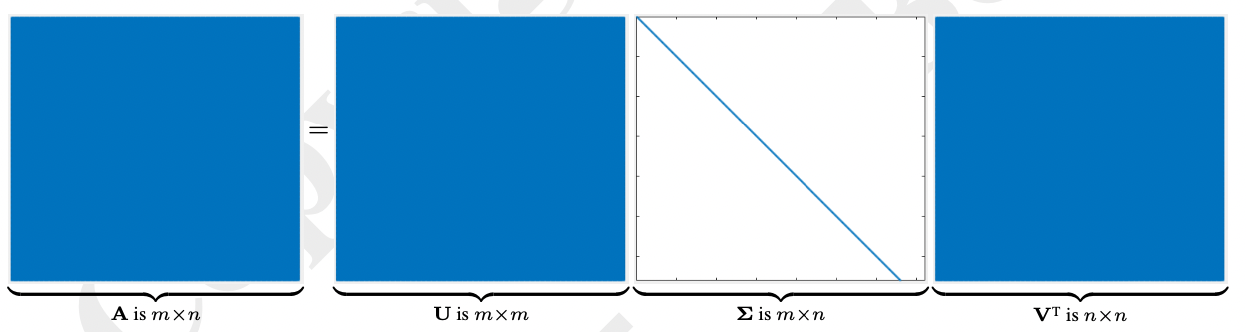
\includegraphics[width=\textwidth]{./imgs/SVD.jpg}
    \caption{SVD Representation of $\mtrA$}
    \label{fig:svdA}
\end{figure}
 As with standard factorization, each of the three matrices tell you information about the parent matrix $\mtrA$. $\mtrSig$  contains the singular values which are the square roots of the eigenvalues of $\matr{A}^T\matr{A}$ and $\mtrV$ represents the associated eigenvectors of those eigenvalues. $\mtrU$ contains the eigenvectors of $\matr{A}\matr{A}^T$. Physically interpreted,  the columns of $\matr{V}$ represent a basis of $\RR^n$ and the columns of $\matr{U}$ represent a basis of $\RR^m$. Written mathematically, this means:
 \begin{align*}
     \mtrA\mvec{x} &= \mtrA( c_1\mvec{V}_1 + c_2\mvec{V}_2 + \dots + c_n\mvec{V}_n)\\
     &= c_1\mtrSig_{11}\mvec{U}_1 +  c_2\mtrSig_{22}\mvec{U}_2 + \dots + c_n\mtrSig_{mm}\mvec{U}_m 
 \end{align*}
